\documentclass[12pt,a4paper]{article}
\usepackage{ctex}
\usepackage{geometry}
\usepackage{graphicx}
\usepackage{setspace}
\usepackage{listings}
\usepackage{listingsutf8}
\usepackage{xcolor}
\usepackage{hyperref}
\usepackage{float} 


\geometry{left=3cm,right=3cm,top=2.5cm,bottom=2.5cm}

% 代码样式
\lstset{
    language=Java,
    inputencoding=utf8,
    basicstyle=\ttfamily\small,
    keywordstyle=\color{blue}\bfseries,
    commentstyle=\color{green!50!black},
    stringstyle=\color{orange},
    showstringspaces=false,
    numbers=left,
    numberstyle=\tiny,
    breaklines=true,
    frame=single
}

\begin{document}

% ================= 封面 =================
\begin{titlepage}
\centering

% 校徽 Logo 
\makebox[\textwidth][c]{%
  
\includegraphics[height=4cm]{fengmian.png}%
}
\vspace*{2cm}

% 学院名称
{\zihao{1}\heiti 信息科学与工程学院}\\[1cm]

% 学年学期
{\zihao{4} 2025---2026 \kaishu学年第一学期}\\[1.5cm]

% 报告标题
\makebox[\textwidth][c]{%
  
\includegraphics[height=2cm]{shiyanbaogao.png}%
}
\\[2em] % 空行
% 实验基本信息表
\zihao{4} 
\renewcommand{\arraystretch}{1.8} % 表格行距
\begin{tabular}{rl}
\heiti 课程名称: & \underline{\makebox[18em][c]{\fangsong Java 编程技术}} \\
\vspace{1cm}
\heiti 实验名称: & \underline{\makebox[18em][c]{\fangsong 循环递归与算法优化}} \\
\kaishu 专  业  班  级 & \underline{\makebox[18em][c]{\kaishu 通信一班}} \\
\kaishu 学  生  学  号 & \underline{\makebox[18em][c]{\kaishu 202300120317}} \\
\kaishu 学  生  姓  名 & \underline{\makebox[18em][c]{\kaishu 陈都阳}} \\
\kaishu 实  验  时  间 & \underline{\makebox[18em][c]{\kaishu 2025年9月16日}} \\
\end{tabular}

\vfill
\end{titlepage}

% ================= 正文 =================
\section*{【实验目的】}
\begin{enumerate}
    \item 熟悉Java的循环递归。
    \item 尝试使用Java来优化复杂度。
\end{enumerate}

\section*{【实验要求】}
\begin{enumerate}
    \item 按要求完成实验一到实验八。
    \item 编译运行,并截图实验结果。
    \item 实验后回答相关思考问题。
\end{enumerate}

\section*{【第一个实验具体内容】}
代码框的问题,代码部分的注释翻译成英文了,原版代码请看附件。
\subsection*{流程图}

\begin{figure}[H]
\centering
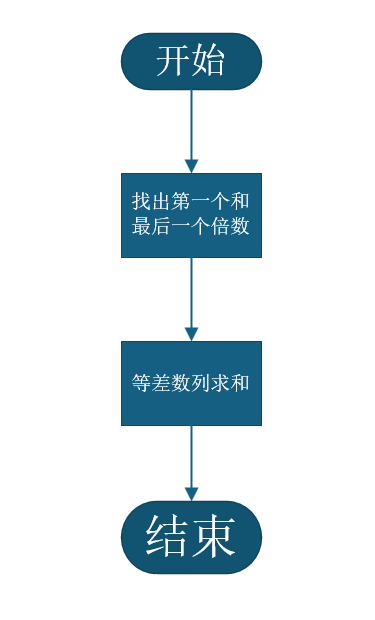
\includegraphics[width=0.8\textwidth]{one1.png}
\caption{流程图}
\end{figure}

\subsection*{部分源代码}
由于代码较长,只显示主要部分,完整代码见附录。
\begin{figure}[H]
\centering
\begin{lstlisting}
// One.java
public void calculateByFormula() {
    // Find the first and last multiples within the range
    int firstMultiple = (start % divisor == 0) ? start : start + (divisor - start % divisor);
    int lastMultiple = end - (end % divisor);
    // If there are no multiples in the range
    if (firstMultiple > end) {
        sum = 0;
        return;
    }
    int count = (lastMultiple - firstMultiple) / divisor + 1;
    sum = count * (firstMultiple + lastMultiple) / 2;
}
public static void main(String[] args) {
    One calculator = new One(1, 2000, 3);
    calculator.calculateByFormula();
    calculator.printResult("Using arithmetic progression formula");
}
\end{lstlisting}
\caption{One 主要部分源代码}
\end{figure}

\subsection*{实验过程与结果}

\begin{figure}[H]
\centering
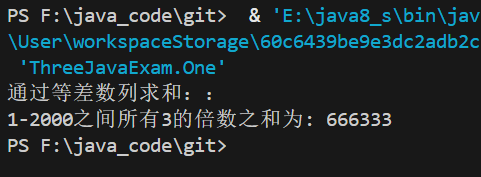
\includegraphics[width=0.8\textwidth]{one.png}
\caption{运行结果}
\end{figure}

\section*{【第二个实验具体内容】}

\subsection*{流程图}

\begin{figure}[H]
\centering
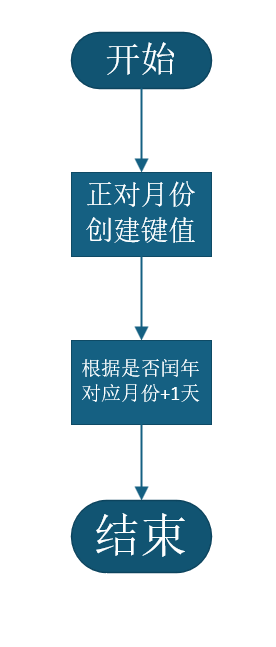
\includegraphics[width=0.5\textwidth]{two1.png}
\caption{流程图}
\end{figure}

\subsection*{部分源代码}
\begin{figure}[H]
\centering
\begin{lstlisting}
// Two.java
public int getDaysByArray() {
    if (month < 1 || month > 12) {
        return -1;
    }
        
    // Array of days in each month (index 0 unused for easy mapping)
    int[] daysInMonth = {0, 31, 28, 31, 30, 31, 30, 31, 31, 30, 31, 30, 31};
        
    // If it's February in a leap year, return 29 days
    if (month == 2 && isLeapYear()) {
        return 29;
    } 
    return daysInMonth[month];
}
public static void main(String[] args) {
    Scanner scanner = new Scanner(System.in);
        
    System.out.println("===== Experiment 2: Date Calculator =====");
    System.out.print("Enter year: ");
    int year = scanner.nextInt();
        
    System.out.print("Enter month (1-12): ");
    int month = scanner.nextInt(); 
    // Create the date calculator object
    Two calculator = new Two(year, month);
        
    // Display detailed information
    calculator.printDetails(); 
    scanner.close();
}



\end{lstlisting}
\caption{TwoQuestion 部分源代码}
\end{figure}

\subsection*{实验过程与结果}

\begin{figure}[H]
\centering
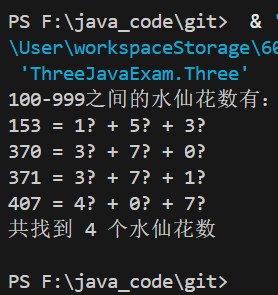
\includegraphics[width=0.8\textwidth]{three.png}
\caption{运行结果}
\end{figure}

\section*{【第三个实验具体内容】}

\subsection*{流程图}

\begin{figure}[H]
\centering
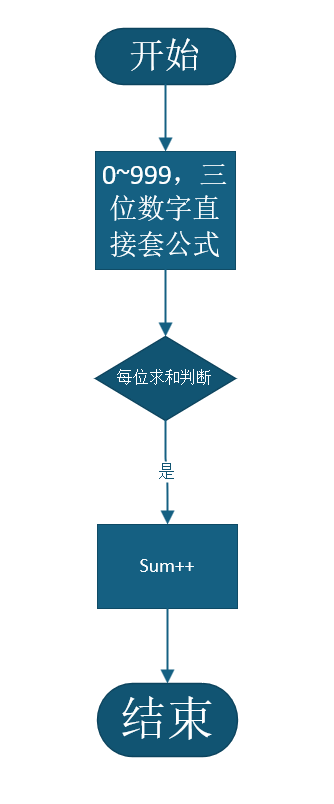
\includegraphics[width=0.5\textwidth]{three1.png}
\caption{流程图}
\end{figure}

\subsection*{部分源代码}
\begin{figure}[H]
\centering
\begin{lstlisting}
// Three.java
public void findAllOptimized() {
    results.clear();

    // Optimization for 3-digit numbers: iterate over each digit directly
    for (int hundreds = 1; hundreds <= 9; hundreds++) {
        for (int tens = 0; tens <= 9; tens++) {
            for (int ones = 0; ones <= 9; ones++) {
                int num = hundreds * 100 + tens * 10 + ones;
                if (num >= start && num <= end) {
                    int sum = hundreds * hundreds * hundreds
                            + tens * tens * tens
                            + ones * ones * ones;
                    if (sum == num) {
                        results.add(num);
                    }
                }
            }
        }
    }
}
public static void main(String[] args) {
    // Function test
    Three finder = new Three(100, 999);
    finder.findAllOptimized();
    finder.printResults();
}

\end{lstlisting}
\caption{ThreeQuestion 部分源代码}
\end{figure}

\subsection*{实验过程与结果}

\begin{figure}[H]
\centering
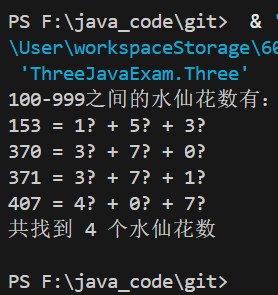
\includegraphics[width=0.8\textwidth]{three.png}
\caption{运行结果}
\end{figure}

\section*{【第四个实验具体内容】}
\subsection*{流程图}

\begin{figure}[H]
\centering
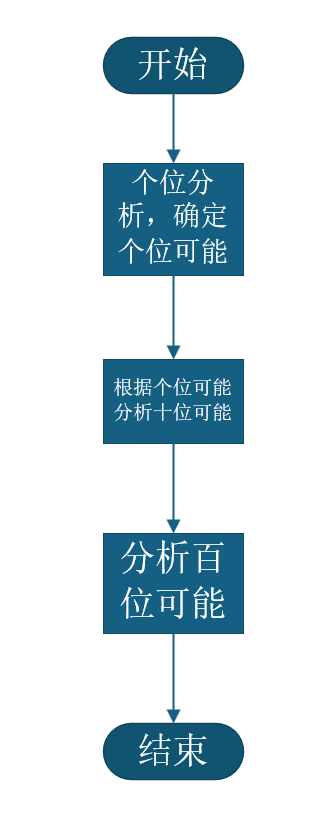
\includegraphics[width=0.5\textwidth]{four1.png}
\caption{流程图}
\end{figure}

\subsection*{部分源代码}
\begin{figure}[H]
\centering
\begin{lstlisting}
// FourQusetion.java
public void solveWithPruning() {
    solutions.clear();
    // Analyze ones place: Z + Z = ?2 (the ones digit of the result is 2)
    // Possible cases: Z = 1 (2), Z = 6 (12 requires carry)
    int[] possibleZ = findPossibleZ();
    for (int z : possibleZ) {
        int carry1 = (z + z) / 10; // carry from ones place
        // Analyze tens place: Y + Z + carry1 = ?3 (the tens digit is 3)
        int[] possibleY = findPossibleY(z, carry1);
        for (int y : possibleY) {
            int carry2 = (y + z + carry1) / 10; // carry from tens place
            // Analyze hundreds place: X + Y + carry2 = 5
            int x = 5 - y - carry2;
            if (x >= 1 && x <= 9) {
                Solution sol = new Solution(x, y, z);
                if (sol.getSum() == targetSum) {
                    solutions.add(sol);
                }
            }
        }
    }
}

\end{lstlisting}

\caption{FourQuestion 部分源代码}
\end{figure}

\subsection*{实验过程与结果}

\begin{figure}[H]
\centering
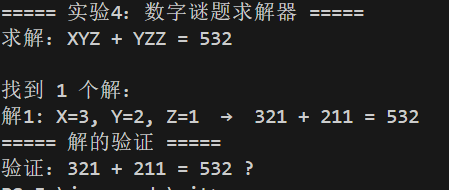
\includegraphics[width=0.8\textwidth]{four.png}
\caption{运行结果}
\end{figure}

\section*{【第五个实验具体内容】}
\subsection*{流程图}

\begin{figure}[H]
\centering
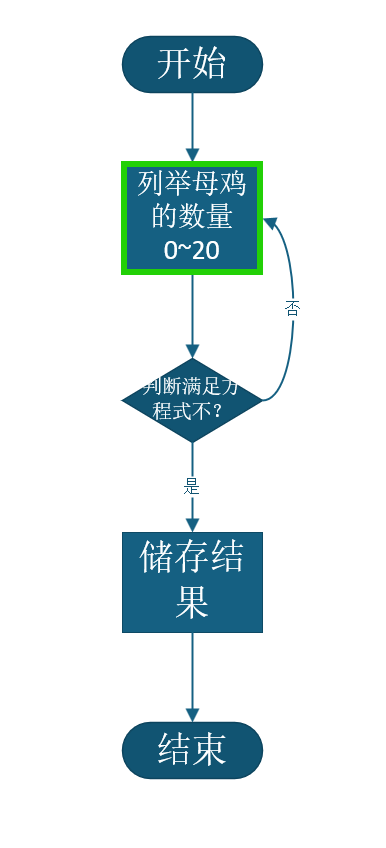
\includegraphics[width=0.7\textwidth]{five1.png}
\caption{流程图}
\end{figure}

\subsection*{部分源代码}
\begin{figure}[H]
\centering
\begin{lstlisting}
// FiveQusetion.java
public void solveOneLoop() {
    solutions.clear();
    // Only need to enumerate the number of hens
    for (int hen = 0; hen <= 20; hen++) {
        if ((100 - 7 * hen) % 4 == 0) {
            int rooster = (100 - 7 * hen) / 4;
            int chick = 100 - hen - rooster;
            if (rooster >= 0 && chick >= 0) {
                PurchasePlan plan = new PurchasePlan(hen, rooster, chick);
                if (plan.isValid()) {
                    solutions.add(plan);
                }
            }
        }
    }
}
public static void main(String[] args) {
    System.out.println("===== Experiment 5: Hundred-Chickens-for-Hundred-Coins Problem =====\n");
    Five solver = new Five();
    System.out.println("Method 3: Single-loop (Optimal)");
    solver.solveOneLoop();
    solver.printSolutions("Method 3: Single-loop (Optimal)");  // Print detailed solutions
}

\end{lstlisting}

\caption{FiveQuestion 部分源代码}
\end{figure}

\subsection*{实验过程与结果}

\begin{figure}[H]
\centering
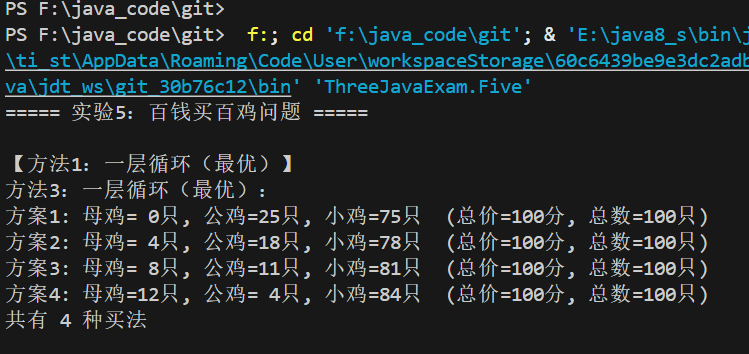
\includegraphics[width=0.8\textwidth]{five.png}
\caption{运行结果}
\end{figure}

\section*{【第六个实验具体内容】}
\subsection*{流程图}

\begin{figure}[H]
\centering
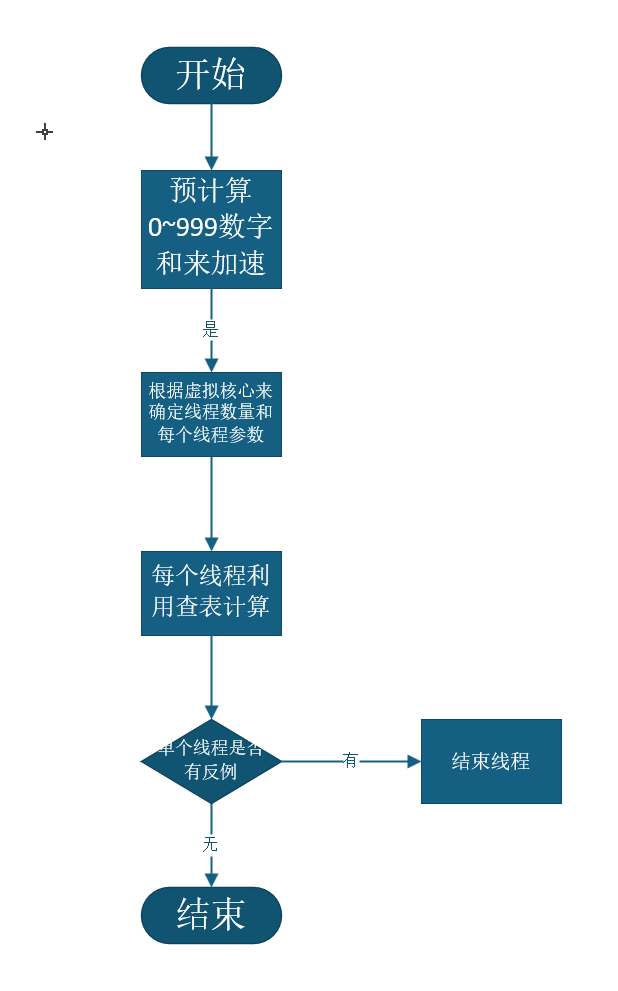
\includegraphics[width=0.5\textwidth]{six1.png}
\caption{流程图}
\end{figure}

\subsection*{部分源代码}
\begin{figure}[H]
\centering
\begin{lstlisting}
// Six.java
public static void main(String[] args) throws InterruptedException {
    int threads = Runtime.getRuntime().availableProcessors() * 2;
    long range = Integer.MAX_VALUE, step = range / threads;
    AtomicBoolean found = new AtomicBoolean(false);
    Thread[] ts = new Thread[threads];
    long start = System.nanoTime();

    for (int t = 0; t < threads; t++) {
        long a = t * step, b = (t == threads - 1) ? range + 1 : (t + 1) * step;
        int id = t;
        ts[t] = new Thread(() -> {
            for (long n = a; n < b && !found.get(); n++) {
                int x = (int) n, mod9 = x % 9, sum = fastSum(x);
                if (sum % 9 == 0 && mod9 != 0 && found.compareAndSet(false, true))
                    System.out.printf("Thread %d found counterexample: n=%d%n", id, x);
            }
        });
        ts[t].start();
    }
    for (Thread t : ts) t.join();
    System.out.printf("Done in %.3f s%n", (System.nanoTime() - start) / 1e9);
}

\end{lstlisting}

\caption{SixQuestion 部分源代码}
\end{figure}

\subsection*{实验过程与结果}
    极限的情况下可以达到0.7s内完成,我觉得大部分功劳是我cpu核心多,而且单独划出24G的内存给虚拟机使用,应该用时间复杂度来衡量优化的效果,单纯的时间不太好说。\\
    
    这道题的最初使用的32线程速度在1.4s左右,后来在思考cpu核心的时候突然想到英特尔的超线程与AMD的并发线程,改用虚拟核心(不在单核单线程)。\\
    
    还有一个优化是我突然想到java自动优化的常量池,我也搞了一个预计算池,直接查表来计算提高了不少。
    预计开启XTU之后可以突破0.5s,后续有时间我去尝试一下。\\
    
    还有一个可以提高的部分是我只是开了单核双线程,实际上考率到线程的上下开销的问题,应该合理调整线程数量,这个得自己一个个测试,后续也可以调整好线程数量后进一步提高性能。\\

\begin{figure}[H]
\centering
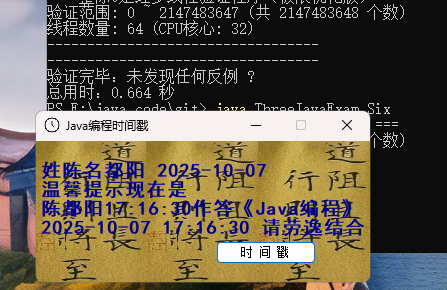
\includegraphics[width=0.8\textwidth]{six.png}
\caption{运行结果}
\end{figure}

\section*{【第七个实验具体内容】}
\subsection*{流程图}

\begin{figure}[H]
\centering
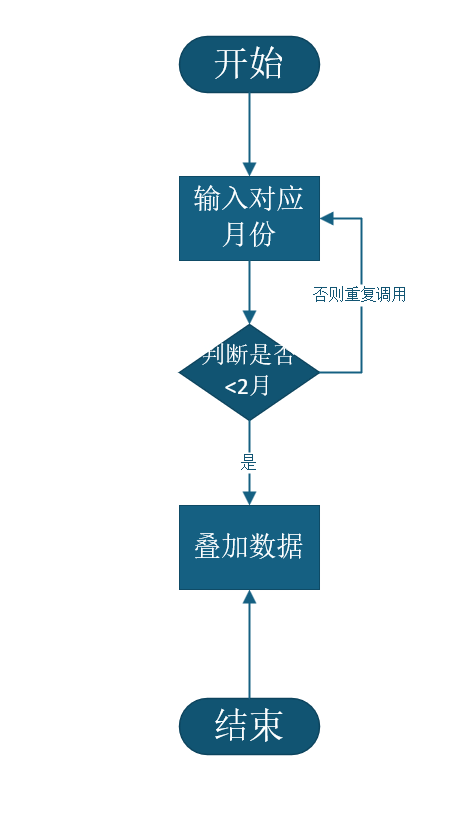
\includegraphics[width=0.8\textwidth]{seven1.png}
\caption{流程图}
\end{figure}

\subsection*{部分源代码}
\begin{figure}[H]
\centering
\begin{lstlisting}
// Seven.java
public static long fibMemo(int n, long[] memo) {
    if (n <= 2) return 1L;
    if (memo[n] != 0) return memo[n];
    memo[n] = fibMemo(n - 1, memo) + fibMemo(n - 2, memo);
    return memo[n];
}
public static void main(String[] args) {
    int months = 24; // 24 months = 2 years
    long[] memo = new long[months + 1];
    long pairs = fibMemo(months, memo);         // Number of rabbit pairs
    long rabbits = pairs * 2;                   // Total number of individual rabbits
    System.out.println("After " + months + " months (2 years):");
    System.out.println("Number of rabbit pairs = " + pairs);
    System.out.println("Total individual rabbits = " + rabbits);
}

\end{lstlisting}

\caption{SevenQuestion 部分源代码}
\end{figure}

\subsection*{实验过程与结果}

\begin{figure}[H]
\centering
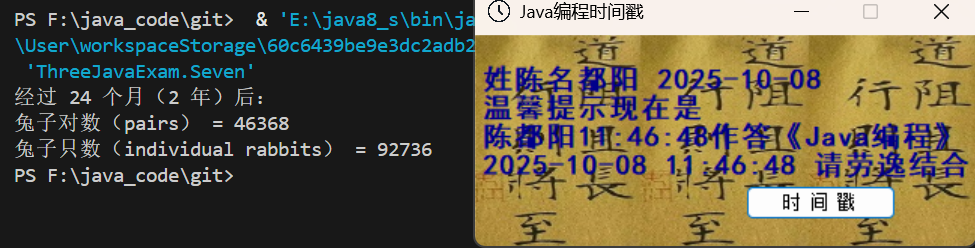
\includegraphics[width=0.8\textwidth]{seven.png}
\caption{运行结果}
\end{figure}
\section*{【第八个实验具体内容】}
\subsection*{流程图}

\begin{figure}[H]
\centering
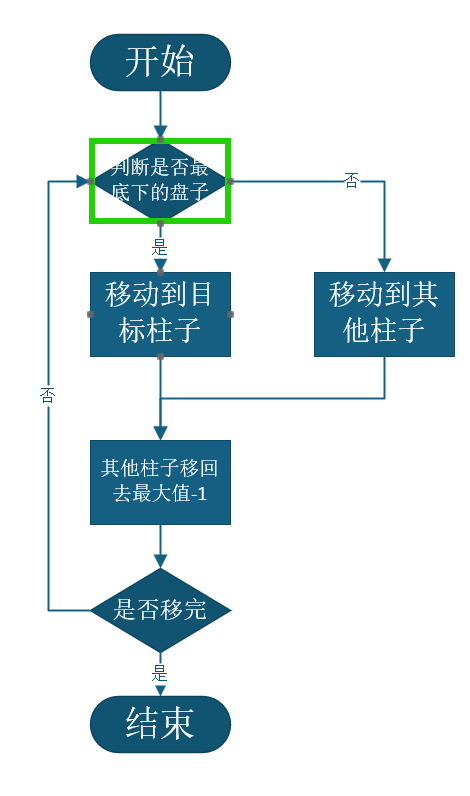
\includegraphics[width=0.8\textwidth]{eight1.png}
\caption{流程图}
\end{figure}

\subsection*{部分源代码}
\begin{figure}[H]
\centering
\begin{lstlisting}
// Enight.java
public static void hanoi(int n, char from, char aux, char to) {
    if (n == 1) {
        System.out.println("Move disk 1: " + from + " -> " + to);
    } else {
        hanoi(n - 1, from, to, aux);
        System.out.println("Move disk " + n + ": " + from + " -> " + to);
        hanoi(n - 1, aux, from, to);
        }
}
public static void main(String[] args) {
    Scanner scanner = new Scanner(System.in);
    System.out.print("Enter the number of disks n: ");
    int n = scanner.nextInt();
    System.out.println("\nSteps to solve the Tower of Hanoi:");
    hanoi(n, 'A', 'B', 'C');
    long steps = (long) Math.pow(2, n) - 1;
    System.out.println("\nTotal moves required: " + steps);
    scanner.close();
}

\end{lstlisting}

\caption{FiveQuestion 部分源代码}
\end{figure}

\subsection*{实验过程与结果}

\begin{figure}[H]
\centering
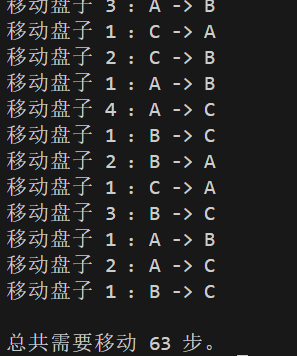
\includegraphics[width=0.8\textwidth]{eight.png}
\caption{运行结果}
\end{figure}

\section*{【实验心得】}
    本次实验主要花费时间在第六个实验的优化上,其他实验都比较简单,主要是考察对基本算法的理解与实现。\\
    
    第六个实验多线程刚开始使用的是从C转过来的代码,刚开始使用的是pthread来管理多线程,后来用着用着老是在3S左右下不来,扒拉了一下数据手册,发现Java的线程管理更简单,直接使用Thread类就可以了。\\
    
    另外一个优化是我突然想到java自动优化的常量池,我也搞了一个预计算池,直接查表来计算提高了不少。\\
    
    我感觉用c语言来验证,套个Java的外壳来调用应该可以压缩一下,时间来不及了,先提交这版实验结果,后面有空再试试搓个C的子程序来试试。\\
    
    而且给的数字2147483647刚好就是int的最大值,应该是有意为之,要是再大一些估计得搞两个int来存。\\

    Java的使用感觉用来大批量流水化搓产品挺不错的,随便翻翻都能翻到自己想要的库,而且有很多现成的算法可以直接拿来用,省去了自己写算法的时间。至于需要优化提速的部分完全可以使用C语言来提速,实在不行还有汇编。不过Java的属性在方法里面调用还是有些小区别的\\
\newpage
\begin{center}
    {\zihao{1}\heiti 附录}
\end{center}
{\zihao{2}【关键字索引】}\\

\setstretch{1.2}
\noindent
\textbf{abstract}:声明抽象类或抽象方法。\\
\textbf{assert}:用于调试时的断言检查。\\
\textbf{boolean}:声明布尔类型变量(true 或 false)。\\
\textbf{break}:跳出当前循环或 switch 语句。\\
\textbf{byte}:声明 8 位有符号整数类型。\\
\textbf{case}:switch 语句中的分支标签。\\
\textbf{catch}:捕获异常。\\
\textbf{char}:声明字符类型(16 位 Unicode)。\\
\textbf{class}:声明一个类。\\
\textbf{const}:保留关键字,未使用。\\
\textbf{continue}:跳过当前循环的剩余部分并进入下一次循环。\\
\textbf{default}:switch 语句中的默认分支。\\
\textbf{do}:与 while 一起使用,构成 do-while 循环。\\
\textbf{double}:声明双精度浮点数类型。\\
\textbf{else}:if 语句的“否则”分支。\\
\textbf{enum}:定义枚举类型。\\
\textbf{extends}:表明一个类继承自另一个类。\\
\textbf{final}:声明常量、不可继承的类或不可重写的方法。\\
\textbf{finally}:定义在异常处理后一定会执行的代码块。\\
\textbf{float}:声明单精度浮点数类型。\\
\textbf{for}:定义 for 循环结构。\\
\textbf{goto}:保留关键字,未使用。\\
\textbf{if}:条件语句的起始关键字。\\
\textbf{implements}:声明一个类实现接口。\\
\textbf{import}:导入包中的类或接口。\\
\textbf{instanceof}:测试对象是否为某个类的实例。\\
\textbf{int}:声明整数类型(32 位)。\\
\textbf{interface}:定义接口。\\
\textbf{long}:声明长整型(64 位)。\\
\textbf{native}:声明一个本地方法(由其他语言实现)。\\
\textbf{new}:创建新对象实例。\\
\textbf{null}:表示空引用。\\
\textbf{package}:定义类所在的包。\\
\textbf{private}:声明私有访问权限。\\
\textbf{protected}:声明受保护访问权限。\\
\textbf{public}:声明公有访问权限。\\
\textbf{return}:从方法返回结果。\\
\textbf{short}:声明 16 位整数类型。\\
\textbf{static}:声明静态成员。\\
\textbf{strictfp}:限制浮点计算的精度和舍入。\\
\textbf{super}:引用父类的成员或构造方法。\\
\textbf{switch}:多分支选择语句。\\
\textbf{synchronized}:声明同步方法或代码块。\\
\textbf{this}:引用当前对象。\\
\textbf{throw}:抛出异常。\\
\textbf{throws}:声明可能抛出的异常类型。\\
\textbf{transient}:声明不被序列化的成员变量。\\
\textbf{try}:定义可能抛出异常的代码块。\\
\textbf{void}:声明方法无返回值。\\
\textbf{volatile}:声明变量在多线程中保持可见性。\\
\textbf{while}:定义 while 循环结构。\\
\textbf{true}、\textbf{false}、\textbf{null}:常量值(非严格意义关键字,但为保留字)。\\
\newpage
{\zihao{2}【代码附录】}\\
\begin{lstlisting}
// One.java
package ThreeJavaExam;

public class One {
    private int start;      // start range
    private int end;        // end range
    private int divisor;    // divisor
    private int sum;        // calculation result
    
    public One(int start, int end, int divisor) {
        this.start = start;
        this.end = end;
        this.divisor = divisor;
        this.sum = 0;
    }
    
    public void calculateByFormula() {
        // Find the first and last multiples in the range
        int firstMultiple = (start % divisor == 0) ? start : start + (divisor - start % divisor);
        int lastMultiple = end - (end % divisor);
        
        // If there are no multiples
        if (firstMultiple > end) {
            sum = 0;
            return;
        }
        int count = (lastMultiple - firstMultiple) / divisor + 1;
        sum = count * (firstMultiple + lastMultiple) / 2;
    }

    public void printResult(String method) {
        System.out.println(method + ":");
        System.out.println("The sum of all multiples of " + divisor + " between " + start + " and " + end + " is: " + sum);
    }

    public static void main(String[] args) {
        One calculator = new One(1, 2000, 3);
        calculator.calculateByFormula();
        calculator.printResult("By arithmetic sequence summation");
    }
}
\end{lstlisting}

\begin{lstlisting}
// Two.java
/**
 * Experiment 2: Determine the number of days in a given year and month
 */
package ThreeJavaExam;

import java.util.Scanner;

public class Two {
    private int year;
    private int month;
    
    /**
     * Constructor
     */
    public Two(int year, int month) {
        this.year = year;
        this.month = month;
    }
    
    /**
     * Check if the year is a leap year
     */
    public boolean isLeapYear() {
        return (year % 4 == 0 && year % 100 != 0) || (year % 400 == 0);
    }
    
    
    /**
     * Optimized method using an array to store days
     */
    public int getDaysByArray() {
        if (month < 1 || month > 12) {
            return -1;
        }
        
        // Array storing days in each month (index 0 unused for direct month correspondence)
        int[] daysInMonth = {0, 31, 28, 31, 30, 31, 30, 31, 31, 30, 31, 30, 31};
        
        // If February and leap year, return 29 days
        if (month == 2 && isLeapYear()) {
            return 29;
        }
        
        return daysInMonth[month];
    }
    
    /**
     * Validate if the month is legal
     */
    public boolean isValidMonth() {
        return month >= 1 && month <= 12;
    }
    
    /**
     * Get the month name in Chinese numerals
     */
    public String getMonthName() {
        return isValidMonth() ? monthNames[month] : "invalid";
    }
    
    /**
     * Print detailed information
     */
    public void printDetails() {
        if (!isValidMonth()) {
            System.out.println("Error: Invalid month!");
            return;
        }
        
        System.out.println("\n===== Date Information =====");
        System.out.println("Year: " + year);
        System.out.println("Is leap year: " + (isLeapYear() ? "Yes" : "No"));
        System.out.println("Number of days: " + getDaysByArray() + " days");
        System.out.println("===================\n");
    }
    
    // Getter and Setter methods
    public int getYear() { return year; }
    public int getMonth() { return month; }
    public void setYear(int year) { this.year = year; }
    public void setMonth(int month) { this.month = month; }
    
    /**
     * Main program entry
     */
    public static void main(String[] args) {
        Scanner scanner = new Scanner(System.in);
        
        System.out.println("===== Experiment 2: Date Calculator =====");
        System.out.print("Please enter the year: ");
        int year = scanner.nextInt();
        
        System.out.print("Please enter the month (1-12): ");
        int month = scanner.nextInt();
        
        // Create date calculator object
        Two calculator = new Two(year, month);
        
        // Display detailed information
        calculator.printDetails();
        
        scanner.close();
    }
}
\end{lstlisting}

\begin{lstlisting}
// Three.java
/**
 * Experiment 3: Narcissistic Number Finder
 */
package ThreeJavaExam;

import java.util.ArrayList;
import java.util.List;

public class Three {
    private int start;      // Search range start
    private int end;        // Search range end
    private List<Integer> results;  // Store found narcissistic numbers
    
    /**
     * Constructor
     */
    public Three(int start, int end) {
        this.start = start;
        this.end = end;
        this.results = new ArrayList<>();
    }
    
    /**
     * Find all narcissistic numbers in the range
     */
    public void findAllOptimized() {
        results.clear();
        
        // Optimization for 100-999: directly iterate through each digit
        for (int hundreds = 1; hundreds <= 9; hundreds++) {
            for (int tens = 0; tens <= 9; tens++) {
                for (int units = 0; units <= 9; units++) {
                    int num = hundreds * 100 + tens * 10 + units;
                    if (num >= start && num <= end) {
                        int sum = hundreds * hundreds * hundreds + tens * tens * tens + units * units * units;
                        if (sum == num) {
                            results.add(num);
                        }
                    }
                }
            }
        } 
    }
    
    /**
     * Get the digit decomposition of a number
     */
    public int[] getDigits(int num) {
        int units = num % 10;
        int tens = (num / 10) % 10;
        int hundreds = num / 100;
        return new int[]{hundreds, tens, units};
    }
    
    /**
     * Print the results
     */
    public void printResults() {
        if (results.isEmpty()) {
            System.out.println("There are no narcissistic numbers between " + start + " and " + end);
            return;
        }
        
        System.out.println("Narcissistic numbers between " + start + " and " + end + " are:");
        for (int num : results) {
            int[] digits = getDigits(num);
            System.out.printf("%d = %d³ + %d³ + %d³%n", 
                            num, digits[0], digits[1], digits[2]);
        }
        System.out.println("Total found: " + results.size() + " narcissistic numbers\n");
    }

    public static void main(String[] args) {
        // Function test
        Three finder = new Three(100, 999);
        finder.findAllOptimized();
        finder.printResults();

    }
}
    
\end{lstlisting}

\begin{lstlisting}
// Four.java
/**
 * Experiment 4: Number Puzzle Solver
 */
package ThreeJavaExam;

import java.util.ArrayList;
import java.util.List;


public class Four {
    
    /**
     * Inner Class: Represents a solution
     */
    public static class Solution {
        private int x, y, z;
        private int xyz, yzz;
        
        public Solution(int x, int y, int z) {
            this.x = x;
            this.y = y;
            this.z = z;
            this.xyz = x * 100 + y * 10 + z;
            this.yzz = y * 100 + z * 10 + z;
        }
        
        public int getX() { return x; }
        public int getY() { return y; }
        public int getZ() { return z; }
        public int getXYZ() { return xyz; }
        public int getYZZ() { return yzz; }
        public int getSum() { return xyz + yzz; }

        public String toString() {
            return String.format("X=%d, Y=%d, Z=%d  →  %d + %d = %d", 
                               x, y, z, xyz, yzz, getSum());
        }
    }
    
    private int targetSum;
    private List<Solution> solutions;
    
    /**
     * Constructor
     */
    public Four(int targetSum) {
        this.targetSum = targetSum;
        this.solutions = new ArrayList<>();
    }
    
    /**
     * Method 1: Solve using carry relationships of units, tens, and hundreds places
     */
    public void solveWithPruning() {
        solutions.clear();
        
        // Analyze units place: Z + Z = ?2 (units digit of result is 2)
        // Possible values: Z=1 (sum=2), Z=6 (sum=12 with carry)
        int[] possibleZ = findPossibleZ();
        
        for (int z : possibleZ) {
            int carry1 = (z + z) / 10;  // Carry from units place
            
            // Analyze tens place: Y + Z + carry1 = ?3 (tens digit of result is 3)
            int[] possibleY = findPossibleY(z, carry1);
            
            for (int y : possibleY) {
                int carry2 = (y + z + carry1) / 10;  // Carry from tens place
                
                // Analyze hundreds place: X + Y + carry2 = 5
                int x = 5 - y - carry2;
                
                if (x >= 1 && x <= 9) {
                    Solution sol = new Solution(x, y, z);
                    if (sol.getSum() == targetSum) {
                        solutions.add(sol);
                    }
                }
            }
        }
    }
    
    private int[] findPossibleZ() {
        List<Integer> possible = new ArrayList<>();
        for (int z = 0; z <= 9; z++) {
            if ((z + z) % 10 == 2) {  // Units digit of sum is 2 after adding Z + Z
                possible.add(z);
            }
        }
        return possible.stream().mapToInt(i -> i).toArray();
    }
    
    private int[] findPossibleY(int z, int carry1) {
        List<Integer> possible = new ArrayList<>();
        for (int y = 1; y <= 9; y++) {
            if ((y + z + carry1) % 10 == 3) {  // Tens digit of sum is 3 after calculation
                possible.add(y);
            }
        }
        return possible.stream().mapToInt(i -> i).toArray();
    }
    
    /**
     * Print all solutions
     */
    public void printSolutions() {
        if (solutions.isEmpty()) {
            System.out.println("No solutions found!");
            return;
        }
        
        System.out.println("Found " + solutions.size() + " solution(s):");
        for (int i = 0; i < solutions.size(); i++) {
            System.out.println("Solution " + (i + 1) + ": " + solutions.get(i));
        }
    }
    
    /**
     * Get list of solutions
     */
    public List<Solution> getSolutions() {
        return new ArrayList<>(solutions);
    }
    
    public static void main(String[] args) {
        System.out.println("===== Experiment 4: Number Puzzle Solver =====");
        System.out.println("Solving: XYZ + YZZ = 532\n");
        
        Four solver = new Four(532);
        
        // Solve using optimized method
        solver.solveWithPruning();
        solver.printSolutions();
        
        // Verify correctness of solutions
        System.out.println("===== Solution Verification =====");
        for (Solution sol : solver.getSolutions()) {
            System.out.printf("Verification: %d + %d = %d %s%n", 
                            sol.getXYZ(), sol.getYZZ(), sol.getSum(),
                            sol.getSum() == 532 ? "✓" : "✗");
        }
    }
}
    
\end{lstlisting}

\begin{lstlisting}
// Five.java
/**
 * Experiment 5: Hundred Coins for Hundred Chickens Problem
 */
package ThreeJavaExam;

import java.util.ArrayList;
import java.util.List;


public class Five {
    
    /**
     * Inner Class: Represents a purchase plan
     */
    public static class PurchasePlan {
        private int hen;        // Number of hens
        private int rooster;    // Number of roosters
        private int chick;      // Number of chicks
        
        // Fixed prices (unit: coins)
        private static final int HEN_PRICE = 5;
        private static final int ROOSTER_PRICE = 3;
        private static final int CHICK_GROUP_PRICE = 1;  // 3 chicks cost 1 coin
        
        public PurchasePlan(int hen, int rooster, int chick) {
            this.hen = hen;
            this.rooster = rooster;
            this.chick = chick;
        }
        
        // Getter methods
        public int getHen() { return hen; }
        public int getRooster() { return rooster; }
        public int getChick() { return chick; }
        
        /**
         * Calculate total number of chickens
         */
        public int getTotalCount() {
            return hen + rooster + chick;
        }
        
        /**
         * Calculate total cost (unit: coins)
         */
        public int getTotalPrice() {
            return hen * HEN_PRICE + rooster * ROOSTER_PRICE + chick / 3;
        }
        
        /**
         * Check if the purchase plan is valid
         * Conditions: total count = 100, total cost = 100, chicks count is divisible by 3
         */
        public boolean isValid() {
            return getTotalCount() == 100 && 
                   getTotalPrice() == 100 && 
                   chick % 3 == 0;
        }

        /**
         * Format plan information as string
         */
        public String toString() {
            return String.format("Hens=%2d, Roosters=%2d, Chicks=%2d  (Total price=%3d coins, Total count=%3d)",
                               hen, rooster, chick, getTotalPrice(), getTotalCount());
        }
    }
    
    private List<PurchasePlan> solutions;  // Store all valid purchase plans
    
    /**
     * Constructor: Initialize solution list
     */
    public Five() {
        this.solutions = new ArrayList<>();
    }

    /**
     * Basic solving method: Triple loop (brute force)
     * Iterate all possible counts of hens, roosters and chicks
     */
    public void solveTripleLoop() {
        solutions.clear();
        
        // Hens can't exceed 20 (100/5)
        for (int hen = 0; hen <= 20; hen++) {
            // Roosters can't exceed 33 (100/3)
            for (int rooster = 0; rooster <= 33; rooster++) {
                // Chicks count is determined (total 100)
                int chick = 100 - hen - rooster;
                
                // Chicks must be non-negative and divisible by 3
                if (chick >= 0 && chick % 3 == 0) {
                    PurchasePlan plan = new PurchasePlan(hen, rooster, chick);
                    if (plan.isValid()) {
                        solutions.add(plan);
                    }
                }
            }
        }
    }
    
    /**
     * Optimized method: Double loop
     * Reduce one loop by calculating chicks count directly
     */
    public void solveDoubleLoop() {
        solutions.clear();
        
        for (int hen = 0; hen <= 20; hen++) {
            // Calculate maximum possible roosters based on remaining money
            int maxRooster = (100 - hen * HEN_PRICE) / ROOSTER_PRICE;
            for (int rooster = 0; rooster <= maxRooster; rooster++) {
                int chick = 100 - hen - rooster;
                if (chick >= 0 && chick % 3 == 0) {
                    PurchasePlan plan = new PurchasePlan(hen, rooster, chick);
                    if (plan.isValid()) {
                        solutions.add(plan);
                    }
                }
            }
        }
    }
    
    /**
     * Optimal solving method: Single loop
     * Derived from mathematical equations to minimize computation
     */
    public void solveOneLoop() {
        solutions.clear();
        
        // Only iterate through possible hen counts (0-20)
        for (int hen = 0; hen <= 20; hen++) {
            // Check if rooster count can be an integer (from equation derivation)
            if ((100 - 7 * hen) % 4 == 0) {
                int rooster = (100 - 7 * hen) / 4;
                int chick = 100 - hen - rooster;
                
                // Ensure non-negative counts
                if (rooster >= 0 && chick >= 0) {
                    PurchasePlan plan = new PurchasePlan(hen, rooster, chick);
                    if (plan.isValid()) {
                        solutions.add(plan);
                    }
                }
            }
        }
    }
    
    /**
     * Print all valid solutions
     *  methodName Name of the solving method to display
     */
    public void printSolutions(String methodName) {
        if (solutions.isEmpty()) {
            System.out.println("No valid solutions found!");
            return;
        }
        
        System.out.println(methodName + ":");
        for (int i = 0; i < solutions.size(); i++) {
            System.out.printf("Solution %d: %s%n", i + 1, solutions.get(i));
        }
        System.out.println("Total " + solutions.size() + " solutions\n");
    }
    
    /**
     * Get copy of solution list (avoid external modification)
     */
    public List<PurchasePlan> getSolutions() {
        return new ArrayList<>(solutions);
    }
    
    /**
     * Main method: Compare different solving methods
     */
    public static void main(String[] args) {
        System.out.println("===== Experiment 5: Hundred Coins for Hundred Chickens Problem =====\n");
        
        Five solver = new Five();

        // Method 1: Triple loop (brute force)
        System.out.println("[Method 1: Triple loop (brute force)]");
        solver.solveTripleLoop();
        solver.printSolutions("Triple loop results");
        
        // Method 2: Double loop (optimized)
        System.out.println("[Method 2: Double loop (optimized)]");
        solver.solveDoubleLoop();
        solver.printSolutions("Double loop results");
        
        // Method 3: Single loop (most efficient)
        System.out.println("[Method 3: Single loop (optimal)]");
        solver.solveOneLoop();
        solver.printSolutions("Single loop results");
    }
}
    
\end{lstlisting}

\begin{lstlisting}
// Six.java
package ThreeJavaExam;

import java.util.concurrent.atomic.AtomicBoolean;

/**
 * Experiment 6: Verify the theorem of divisibility by 9
 */
public class Six {  
    // Precompute the sum of digits for 0-999
    private static final int[] DIGIT_SUM_CACHE = new int[1000];
    
    static {
        for (int i = 0; i < 1000; i++) {
            int sum = 0;
            int n = i;
            while (n > 0) {
                sum += n % 10;
                n /= 10;
            }
            DIGIT_SUM_CACHE[i] = sum;
        }
    }

    public static void main(String[] args) throws InterruptedException {
        // Number of threads and range
        final int THREAD_COUNT = Runtime.getRuntime().availableProcessors() * 2; // Dynamically adjust
        final long RANGE = (long) Integer.MAX_VALUE;
        final long STEP = RANGE / THREAD_COUNT;

        System.out.println("Verification range: 0 ~ " + RANGE + " (total " + (RANGE + 1) + " numbers)");
        System.out.println("Number of threads: " + THREAD_COUNT + " (CPU cores: " + Runtime.getRuntime().availableProcessors() + ")");

        AtomicBoolean found = new AtomicBoolean(false);
        Thread[] threads = new Thread[THREAD_COUNT];
        long startTime = System.nanoTime();

        for (int t = 0; t < THREAD_COUNT; t++) {
            final int threadId = t;
            final long start = t * STEP;
            final long end = (t == THREAD_COUNT - 1) ? RANGE + 1 : (t + 1) * STEP;  // +1 to include maximum value

            threads[t] = new Thread(() -> {
                // Core mathematical principle: n % 9 == digitSum(n) % 9
                // So we only need to verify if this equation always holds
                for (long n = start; n < end && !found.get(); n++) {
                    int num = (int) n;
                    
                    // Skip obviously valid cases (multiples of 9)
                    int mod9 = num % 9;
                    if (mod9 == 0) continue; // For multiples of 9, sum of digits must be a multiple of 9
                    
                    // Quickly calculate sum of digits (using lookup table)
                    int sum = fastDigitSum(num);
                    int sumMod9 = sum % 9;
                    
                    // Check if the theorem is violated
                    if (sumMod9 == 0 && mod9 != 0) {
                        if (found.compareAndSet(false, true)) {
                            System.out.printf("Thread %d found a counterexample! n=%d sum of digits=%d (sum%%9==0, but n%%9=%d)%n",
                                    threadId, num, sum, mod9);
                        }
                        return;
                    }
                }
            });
            threads[t].start();
        }

        // Wait for all threads to complete
        for (Thread thread : threads) {
            thread.join();
        }

        long time = System.nanoTime() - startTime;
        System.out.println("----------------------------------");
        if (found.get())
            System.out.println("Verification terminated early: counterexample found ");
        else
            System.out.println("Verification completed: no counterexamples found ");
        System.out.printf("Total time: %.3f seconds%n", time / 1_000_000_000.0);
    }

    /**
     * Calculate using precomputed table
     */
    private static int fastDigitSum(int n) {
        if (n < 1000) {
            return DIGIT_SUM_CACHE[n];
        }
        
        int sum = 0;
        
        // Process in segments: handle 3 digits each time
        while (n >= 1000) {
            int last3 = n % 1000;
            sum += DIGIT_SUM_CACHE[last3];
            n /= 1000;
        }
        
        // Process remaining part
        sum += DIGIT_SUM_CACHE[n];
        
        return sum;
    }
}
\end{lstlisting}

\begin{lstlisting}
// Seven.java
package ThreeJavaExam;

public class Seven {

    /**
     * Calculates Fibonacci number using memoization (recursive approach)
     */
    public static long fibMemo(int n, long[] memo) {
        // Base case: 1 pair of rabbits in the 1st and 2nd months
        if (n <= 2) return 1L;            
        // Return cached value if already computed
        if (memo[n] != 0) return memo[n];
        // Recursively calculate and store result in memo array
        memo[n] = fibMemo(n - 1, memo) + fibMemo(n - 2, memo);
        return memo[n];
    }

    public static void main(String[] args) {
        int months = 24; // Target period: 24 months

        // Memoization array: index represents month, value represents rabbit pairs
        long[] memo = new long[months + 1];
        long rabbitPairs = fibMemo(months, memo);         // Calculate number of rabbit pairs
        long rabbitIndividuals = rabbitPairs * 2;         // Convert pairs to individuals (1 pair = 2 rabbits)

        System.out.println("After " + months + " months (2 years):");
        System.out.println("Number of rabbit pairs = " + rabbitPairs);
        System.out.println("Number of individual rabbits = " + rabbitIndividuals);
    }
}
    
\end{lstlisting}

\begin{lstlisting}
// Eight.java
package ThreeJavaExam;

import java.util.Scanner;

public class Enight {

    /**
     * Implement Tower of Hanoi recursively
     */
    public static void hanoi(int n, char from, char aux, char to) {
        if (n == 1) {
            System.out.println("Move disk 1: " + from + " -> " + to);
        } else {
            // First move the top n-1 disks from source to auxiliary
            hanoi(n - 1, from, to, aux);
            // Then move the largest disk from source to target
            System.out.println("Move disk " + n + ": " + from + " -> " + to);
            // Finally move the n-1 disks from auxiliary to target
            hanoi(n - 1, aux, from, to);
        }
    }

    /**
     * Main function: read input and call recursive function
     */
    public static void main(String[] args) {
        Scanner scanner = new Scanner(System.in);

        System.out.print("Please enter the number of disks n: ");
        int n = scanner.nextInt();

        System.out.println("\nTower of Hanoi movement steps:");
        hanoi(n, 'A', 'B', 'C');

        // Total steps formula: 2^n - 1
        long steps = (long) Math.pow(2, n) - 1;
        System.out.println("\nTotal steps required: " + steps + ".");

        scanner.close();
    }
}
    
\end{lstlisting}

\end{document}

